\documentclass{article}

\usepackage{tikz}

\begin{document}

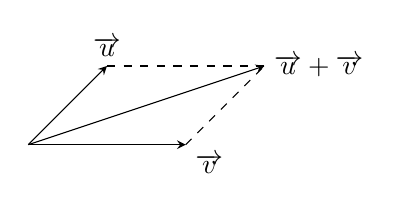
\begin{tikzpicture}[>=stealth]
  \draw[->] (0,0)-- (1,1) node[above]{$\overrightarrow{u}$};
  \draw[->] (0,0)-- (2,0) node[below right]{$\overrightarrow{v}$}; 
  \draw [->] (0,0)-- (3,1);
  \draw[dashed] (1,1)-- (3,1);
  \draw[dashed] (2,0)-- (3,1) node[right]
      {$\overrightarrow{u}+ \overrightarrow{v}$};
\end{tikzpicture}
\qquad
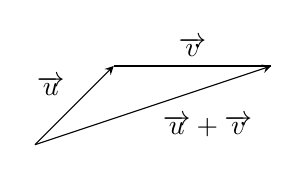
\begin{tikzpicture}[>=stealth]
  \draw[->] (0,0)-- (1,1) node[midway,above left]{$\overrightarrow{u}$};
  \draw [->] (0,0)-- (3,1) node[midway, below right]
    {$\overrightarrow{u} + \overrightarrow{v}$};
  \draw (1,1)-- (3,1 ) node[midway, above] {$\overrightarrow{v}$};
\end{tikzpicture}

\end{document}
